\documentclass[12pt]{article}
\usepackage[top=1in,left=1in, right = 1in, footskip=1in]{geometry}

\usepackage{graphicx}
%\usepackage{adjustbox}

\newcommand{\eref}[1]{(\ref{eq:#1})}
\newcommand{\fref}[1]{Fig.~\ref{fig:#1}}
\newcommand{\Fref}[1]{Fig.~\ref{fig:#1}}
\newcommand{\sref}[1]{Sec.~\ref{#1}}
\newcommand{\frange}[2]{Fig.~\ref{fig:#1}--\ref{fig:#2}}
\newcommand{\tref}[1]{Table~\ref{tab:#1}}
\newcommand{\tlab}[1]{\label{tab:#1}}
\newcommand{\seminar}{SE\mbox{$^m$}I\mbox{$^n$}R}

\usepackage{amsthm}
\usepackage{amsmath}
\usepackage{amssymb}
\usepackage{amsfonts}

\usepackage{lineno}
%\linenumbers

\usepackage[pdfencoding=auto, psdextra]{hyperref}

\bibliographystyle{chicago}
\usepackage{natbib}
\date{\today}

\usepackage{xspace}
\newcommand*{\ie}{i.e.\@\xspace}

\usepackage{color}

\newcommand{\Rx}[1]{\ensuremath{{\mathcal R}_{#1}}} 
\newcommand{\Ro}{\Rx{0}}
\newcommand{\RR}{\ensuremath{{\mathcal R}}}
\newcommand{\Rhat}{\ensuremath{{\hat\RR}}}
\newcommand{\tsub}[2]{#1_{{\textrm{\tiny #2}}}}
\newcommand{\dd}[1]{\ensuremath{\, \mathrm{d}#1}}

\newcommand{\comment}[3]{\textcolor{#1}{\textbf{[#2: }\textsl{#3}\textbf{]}}}
\newcommand{\jd}[1]{\comment{cyan}{JD}{#1}}
\newcommand{\swp}[1]{\comment{magenta}{SWP}{#1}}
\newcommand{\dc}[1]{\comment{blue}{DC}{#1}}
\newcommand{\hotcomment}[1]{\comment{red}{HOT}{#1}}

\newcommand{\jdnew}{\jd{NEW}}
\newcommand{\jddel}[1]{\jd{DELETE: #1}}

\begin{document}

\begin{flushleft}{
	\Large
	\textbf\newline{
	Supplementary Materials for Predicting the impact of non-pharmaceutical interventions against COVID-19 on \textit{Mycoplasma pneumoniae} in the United States
	}
}
\newline
\\ 
Sang Woo Park\textsuperscript{1,2,*}, Brooklyn Noble\textsuperscript{3}, Emily Howerton\textsuperscript{1}, Bjarke F Nielsen\textsuperscript{4}, Sarah Lentz\textsuperscript{3}, Lilliam Ambroggio\textsuperscript{5}, Samuel Dominguez\textsuperscript{6}, Kevin Messacar\textsuperscript{6}, Bryan T Grenfell\textsuperscript{1}
\\
\bigskip
\textbf{1} Department of Ecology and Evolutionary Biology, Princeton University, Princeton, NJ, USA
\\
\textbf{2} Department of Ecology and Evolution, University of Chicago, Chicago, IL, USA
\\
\textbf{3} bioMérieux, Salt Lake City, Utah, USA
\\
\textbf{1} Department of Ecology and Evolutionary Biology, Princeton University, Princeton, NJ, USA
\\
\textbf{4} High Meadows Environmental Institute, Princeton University, Princeton, New Jersey, USA
\\
\textbf{5} Department of Pediatrics, Sections of Emergency Medicine and Hospital Medicine, University of Colorado School of Medicine and Children's Hospital Colorado, Aurora, CO, USA
\\
\textbf{6} Department of Pediatrics, Section of Infectious Diseases, University of Colorado School of Medicine and Children's Hospital Colorado, Aurora, CO, USA
\\
\bigskip

*Corresponding author: swp2@uchicago.edu
\bigskip
\end{flushleft} 

\pagebreak

\setcounter{figure}{0}
\setcounter{equation}{0}
\renewcommand{\thefigure}{S\arabic{figure}}
\renewcommand{\theequation}{S\arabic{equation}}

\section*{Supplementary Figures}

\begin{figure}[!ht]
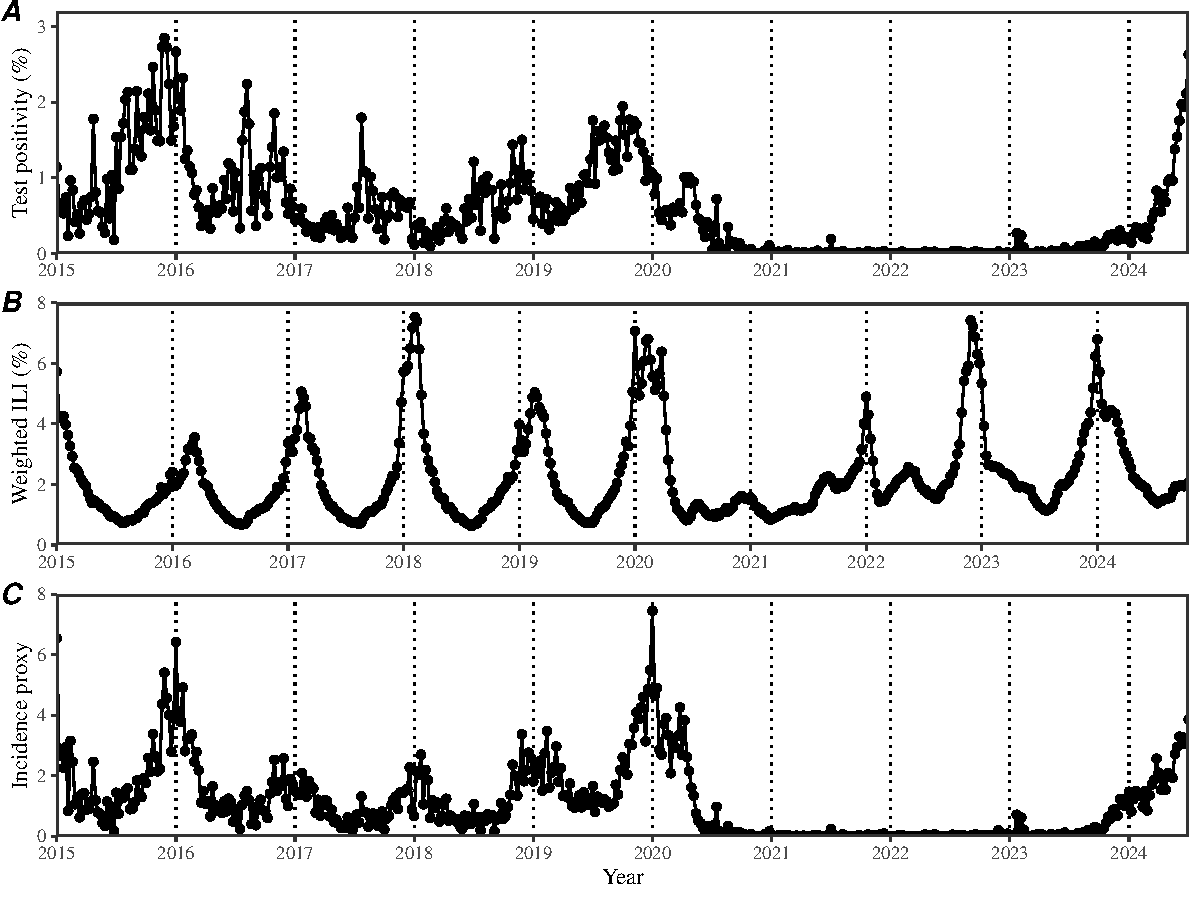
\includegraphics[width=\textwidth]{../figure_timeseries/figure_timeseries.pdf}
\caption{
\textbf{Comparisons of time series data.}
(A) Weekly percent positivity of Mp infections BIOFIRE\textsuperscript{®} Respiratory Panel in the US.
(B) Weekly percent positivity of outpatient visits for ILI in the US.
(C) Estimated weekly incidence proxy.
}
\end{figure}

\pagebreak

\begin{figure}[!ht]
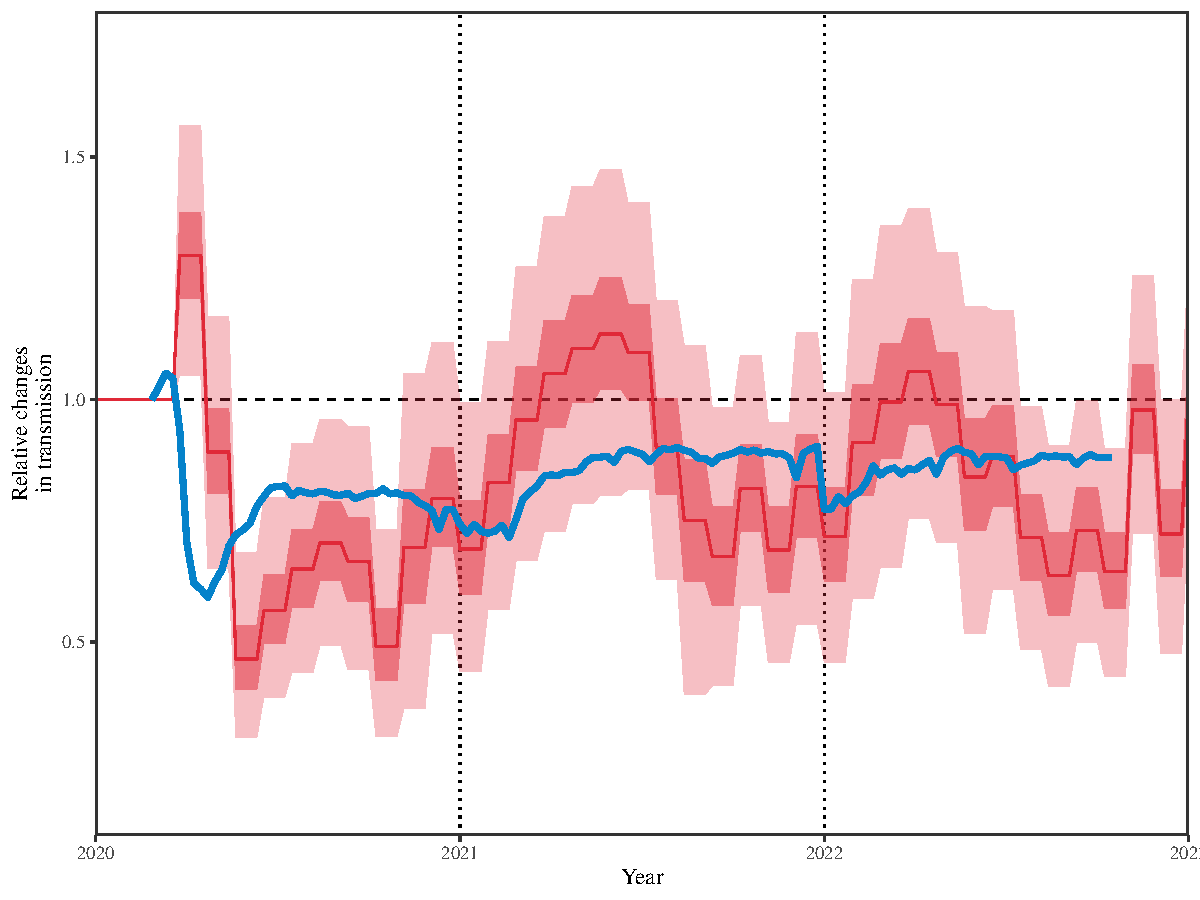
\includegraphics[width=\textwidth]{../figure_mobility/figure_mobility_new.pdf}
\caption{
\textbf{Comparisons of estimated changes in transmission (red) and mean Google mobility measures (blue).}
Mean mobility was calculated by taking the average mobility across four categories: retail \& recreation, grocery \& pharmacy, transit stations, and workplaces \citep{park2024predicting}.
}
\end{figure}


\pagebreak

\begin{figure}[!ht]
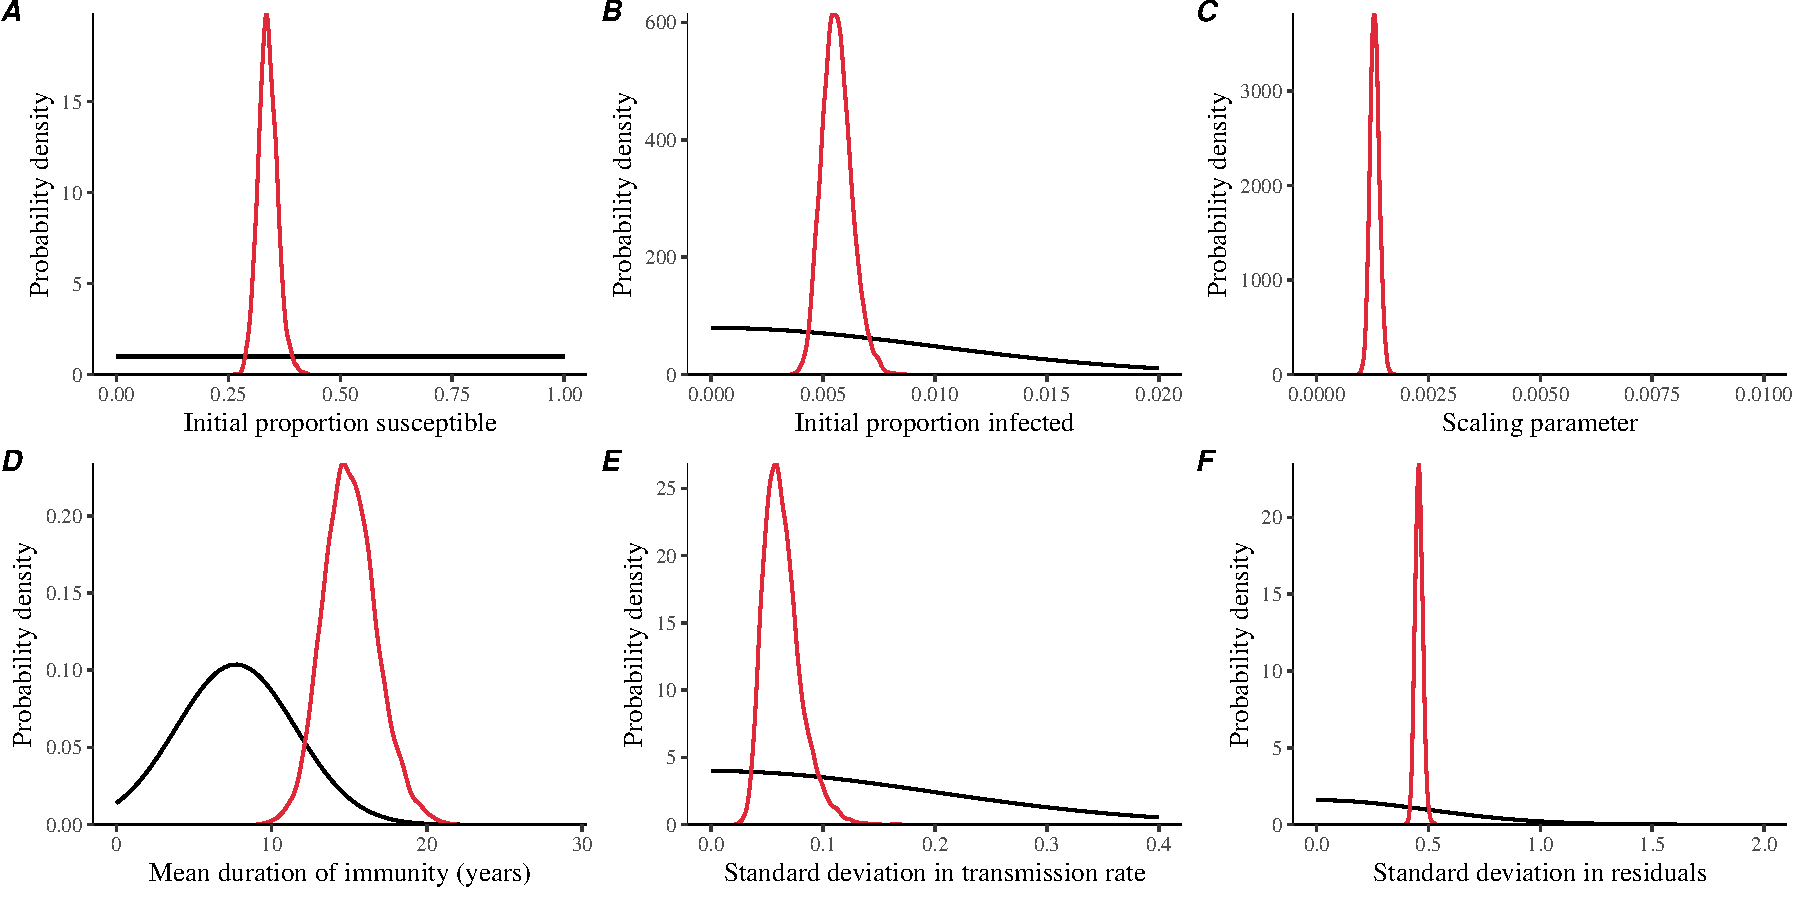
\includegraphics[width=\textwidth]{../figure1/figure1_posterior.pdf}
\caption{
\textbf{Comparisons between posterior and prior distributions.}
Black lines represent prior distributions.
Red lines represent posterior distributions.
Posterior distributions for the seasonal transmission rate and NPI effects are presented in Figure 1.
Note that the prior distribution for the scaling parameter is not visible in panel C because the assumed distribution is much wider (a half normal with a mean of 0 and standard deviation of 2) and therefore has much lower densities.
}
\end{figure}

\pagebreak

\begin{figure}[!ht]
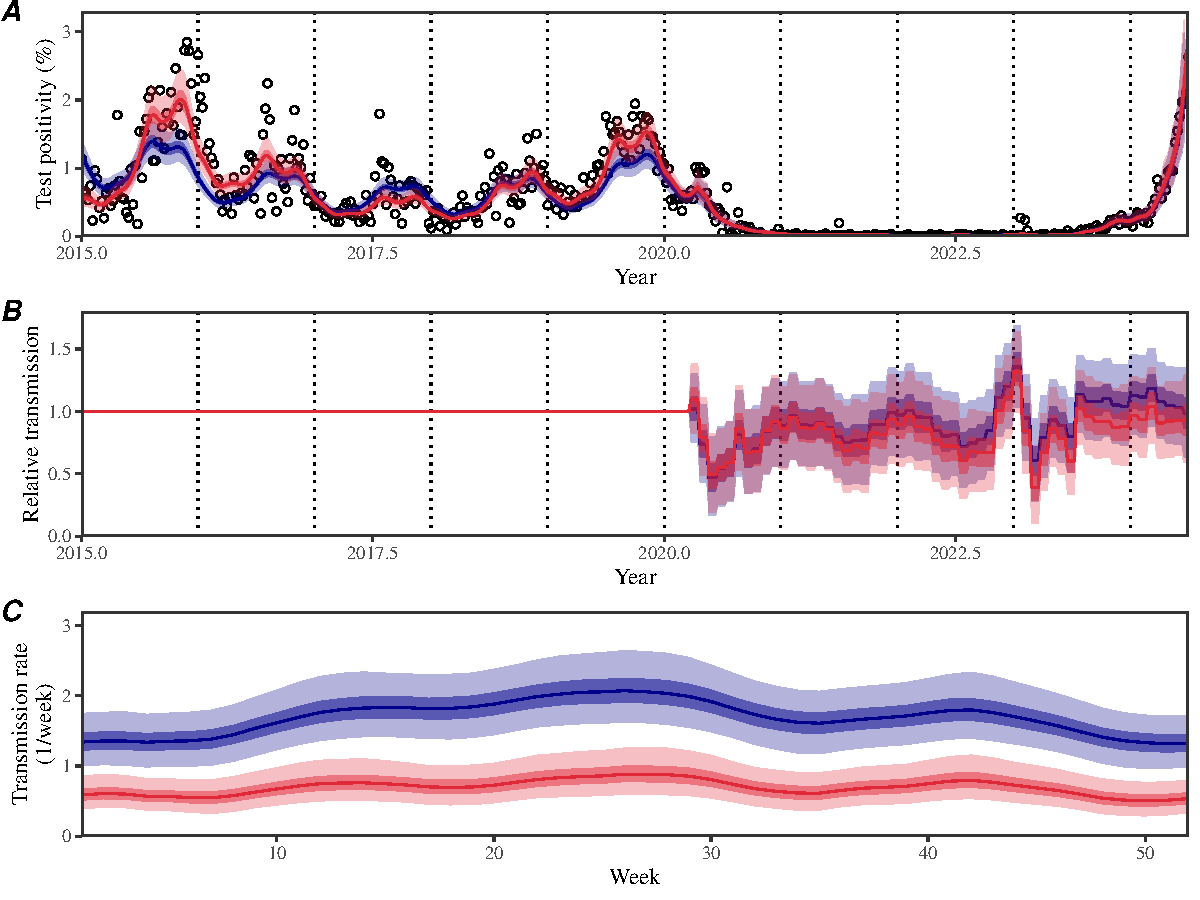
\includegraphics[width=\textwidth]{../figure_sirs/figure_sirs_fit.pdf}
\caption{
\textbf{Comparisons of SIRS (red) and SIR (blue) model fits to Mycoplasma pneumoniae positivity in the US, 2015--2024.}
(A) Comparisons of observed (points) and fitted (line) changes in weekly test positivity for Mp infections.
(B) Estimated non-periodic, time-varying transmission term, representing relative transmission $\delta$ following the introduction of NPIs.
These changes are relative to the seasonal transmission rate shown in panel C;
for example, 0.5 corresponds to a 50\% reduction in transmission.
(C) Estimated periodic transmission term  $\tsub{\beta}{seas}(t)$, representing seasonal transmission rate.
Lines and shaded regions represent the estimated posterior median and corresponding 95\% and 50\% credible intervals.
}
\end{figure}

\pagebreak

\begin{figure}[!ht]
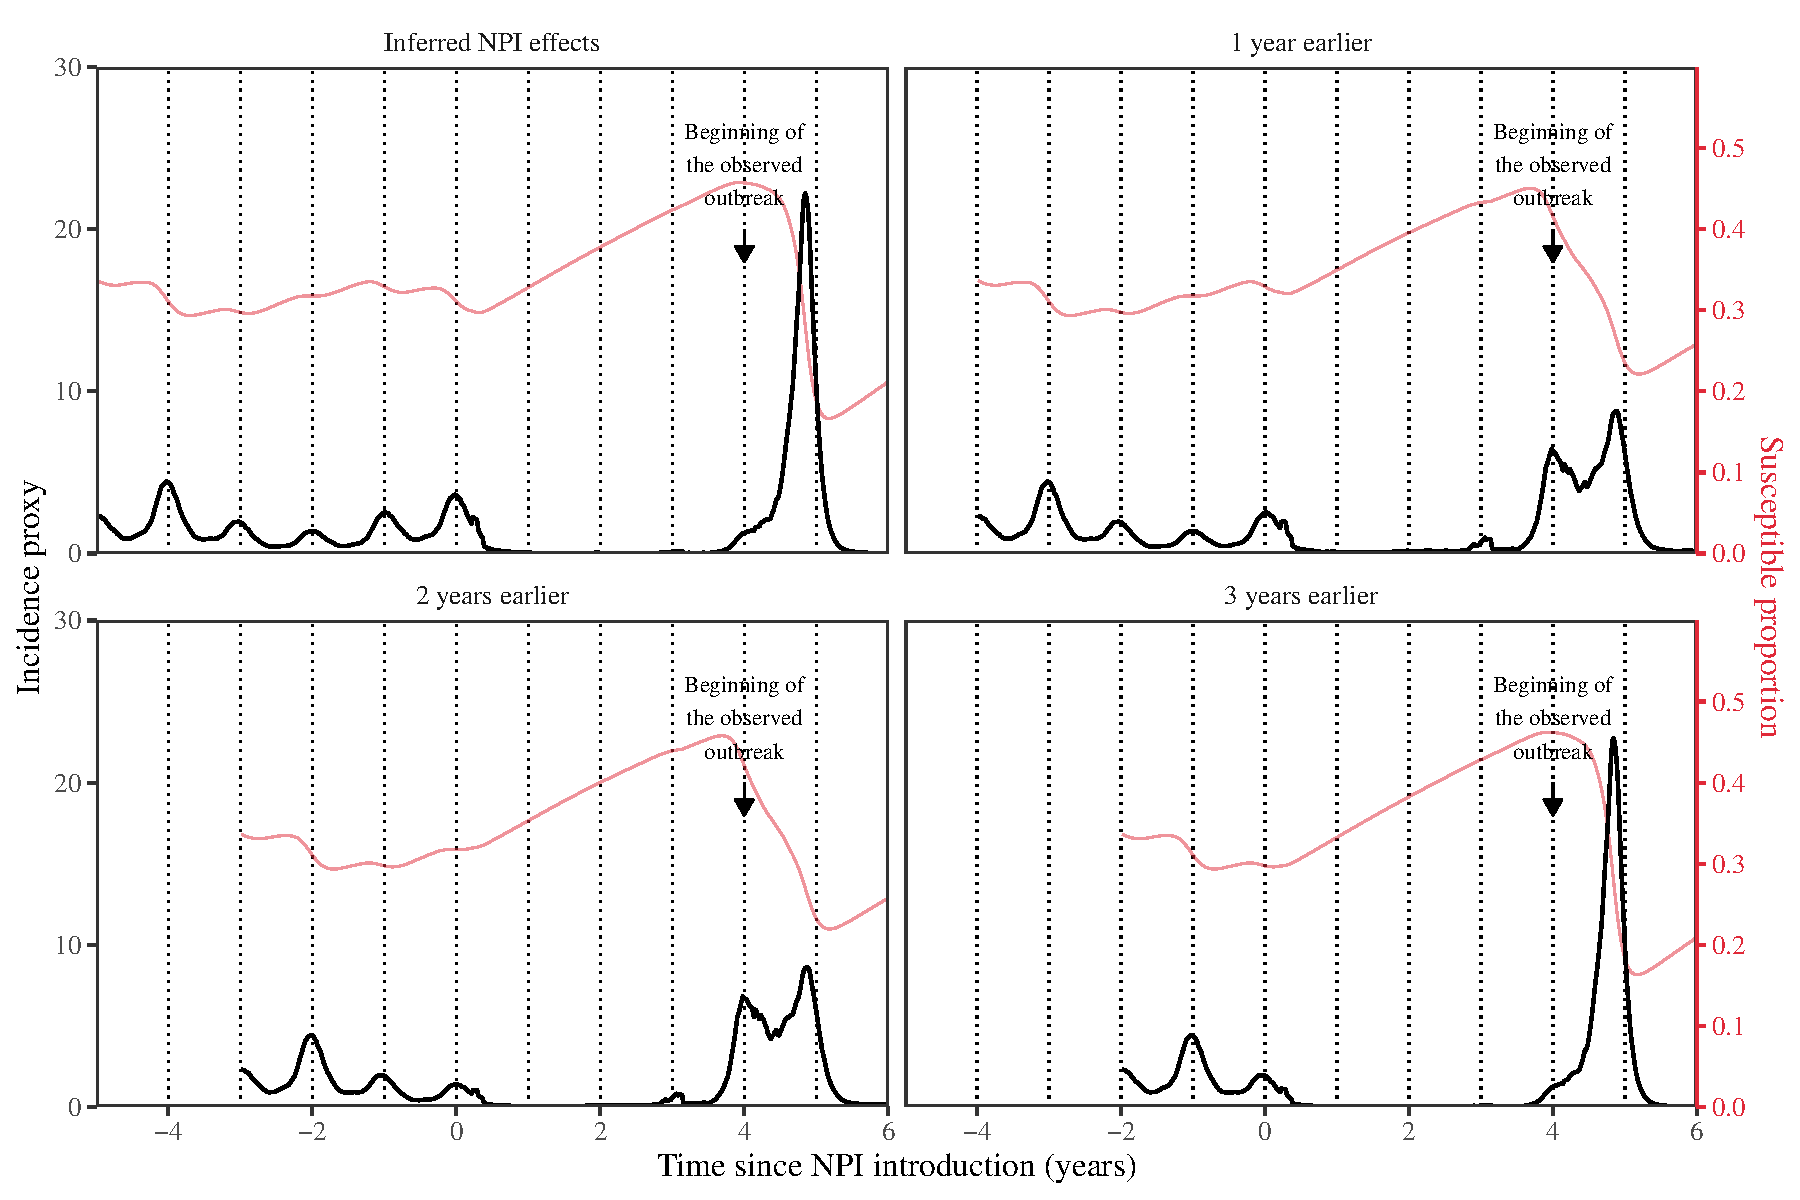
\includegraphics[width=\textwidth]{../figure3/figure3_cyclic.pdf}
\caption{
\textbf{Impact of timing of NPI introduction, relative to the timing of the multiannaul cycles of Mp outbreaks.}
Sensitivity analyses were performed by shifting the estimated $\delta$ by 1--3 years to explore counterfactual scenarios that allow earlier introduction of NPIs.
The first panel (inferred NPI effects) represent our main predictions (shown in Figure 2 in the main text) following the observed epidemic.
All other panels represent counterfactual simulations.
Black lines represent the predicted incidence proxy.
Red lines represent the predicted susceptible proportion.
}
\end{figure}

\pagebreak

\bibliography{myco}

\end{document}
